\chapter{Collaborative Tasks}
\label{chapter:colab-tasks}

\par Em cada task falar do processo teórico que leva a execução da tarefa 

\section{Hand Guiding}

\par Explain how to go from wrench\_forces to global ee\_velocity

\par Explain here the conversion from eef\_velocity to o joint speed. say that here is the first time that this conversion is talked about 

% ADD: Reference this subsection from other places mainly end of chapter 3 and 4

\begin{figure}[h]
    \centering
    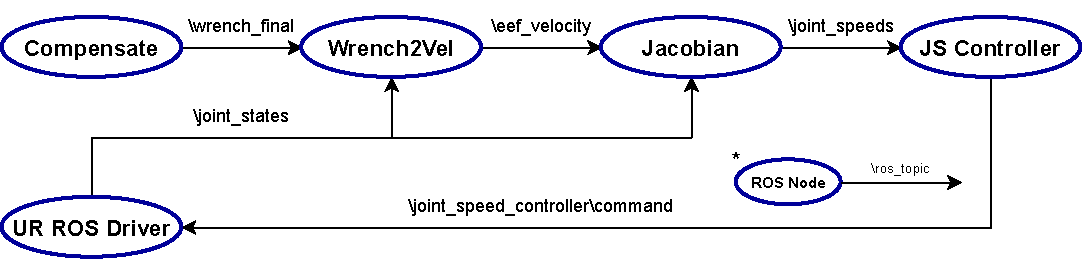
\includegraphics[width=\linewidth]{figs/chp4/ros_hg_arch.pdf}
    \caption{\ac{ros} architecture of the \ac{hg} task}
    \label{fig:ros_hg_arch}
\end{figure}

\section{Object Transfer}

\par Explain the execution of this task... explain the importance of a parametrized skill because the user can define the pick and deliver place and the task works every time
\par explain the intrinsic details of the deliver method

\section{Object Lifting Assistance}

\par This task is more complex, since after gripping a lot of things happen, the controllers are switched, the robot is moved 5 cm upwards to make the user not interact with the gripper beacuse it will calibrate the weight, after the weight is calibrated the hand guide feature is back online with the new calibrated weight on the ft theory model... the robot will continue in hand guide until a double tap on y is perform, making the robot release the object and set the weight to zero... when the robot releases the weight it will also zero de ft sensor because as said previously, interactiong with the sensor can cause deveiations on the measurements

\section{Collision Free Execution of an Industrial Task}

\par definition of an industrial task, turn on collision avoidacne algorithm, now the joint speed controller will listen to the pf controller and the robot will be performing the task until an interaction is made with it

\section{Collaborative State Machine}

\par explain the intrinsic detail of the state machine
\par good for overall system architecture and description of the state machine


\subsection{State Transitions}

\par explain here the double tap interaction

\subsection{Visual Feedback}

\par explain here the gripper color changing intergation


\section{Software Tools for \acs{hrc}}
\label{sec:tools-hrc}

\par iris\_sami
\par iris\_cobot
\par other viewers and tools such as plotjuggler integration and smach\_viewer
